\documentclass[titlepage]{article}
\usepackage{babel}
\usepackage{amsmath}
\usepackage{amssymb}
\usepackage{amsthm}
\usepackage{multicol} %spalten in seite
\usepackage{graphicx} %bilder einfügen
\usepackage[normalem]{ulem} %durchstreichen
\usepackage{tabto} %tabulator mit \tab
\usepackage{hyperref}
\usepackage{wasysym}
\usepackage{bbm}
\usepackage{bbold}
\usepackage{svg}
\usepackage{xcolor}
\usepackage[T1]{fontenc}
\usepackage{mathrsfs}  
\usepackage[utf8]{inputenc}
\usepackage{listings} %quellcode
\pagestyle{plain}
\pagenumbering{arabic}
\renewcommand{\arraystretch}{1.3} %vertikaler abstand von tabellen
\newcommand{\n}{\newline}
\usepackage[left=20mm, right=15mm, top=25mm, bottom=30mm, paper=a4paper]{geometry}
\renewcommand{\contentsname}{Inhaltsverzeichnis}

\newcommand{\K}{\mathbb{K}}
\newcommand{\C}{\mathbb{C}}
\newcommand{\N}{\mathbb{N}}
\newcommand{\Q}{\mathbb{Q}}
\newcommand{\R}{\mathbb{R}}
\newcommand{\1}{\mathbb{1}}
\newcommand{\0}{\mathbb{0}}
\newcommand{\Z}{\mathbb{Z}}
\renewcommand{\P}{\mathscr{P}}
\newcommand{\tb}{\textbackslash}

\begin{document}
	
	\title{Diskrete Strukturen - Übung 07}
	\author{Felix Tischler, Martrikelnummer: 191498}
	\date{\today}
	\maketitle
	
	\part*{Mengen}
	\section*{1.) $Es$ $gibt$ $ein$ $Venn-Diagramm$ $aus$ $drei$ $sich$ $überschneidenden$ $Kreisen,$ $das$ $alle$	$m\ddot oglichen$ $acht$ $F\ddot alle$ $zeigt,$ $in$ $denen$ $sich$ $ein$ $Objekt$ $in$ $Bezug$ $auf$ $drei$ $Mengen$	$befinden$ $kann.$}
		\subsection*{a) $Zeichnen$ $Sie$ $ein$ $solches$ $Venn-Diagramm$ $mit$ $drei$ $Mengen$ $A, B, C.$ $Beschreiben$ $Sie$ $die$ $acht$ $F\ddot alle$ $mit$ $Hilfe$ $der$ $Mengenoperationen$ $\cap,\cup,\bar\,$.}
		\begin{figure}[htbp]
			\centering
			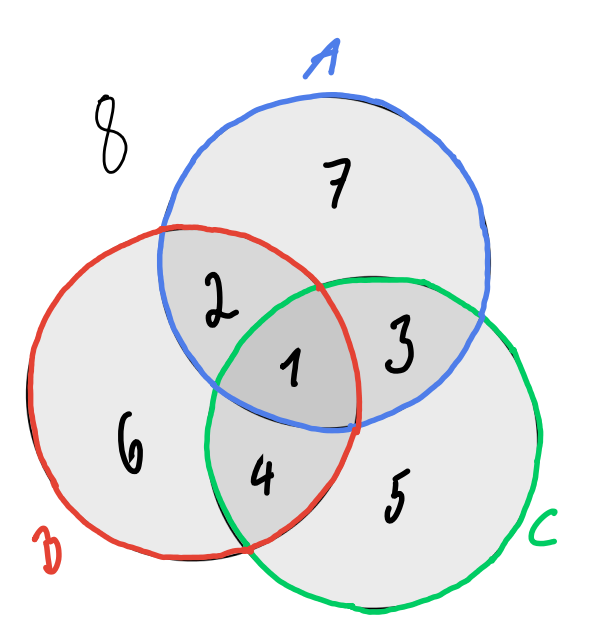
\includegraphics[width=7cm,height=7cm]{venn37.png}
			\caption{Venn-Diagramm mit 3 Mengen}
		\end{figure}
			\noindent
			\begin{center}
				\centering
				$1:=A\cap B\cap C,$ $2:=A\cap B\cap\bar C,$ $3:=A\cap C\cap\bar B,$ $4:=\bar A\cap B\cap C,$\\$5:=\bar A\cap\bar B\cap C,$ $6:=\bar A\cap B\cap\bar C,$ $7:=A\cap\bar B\cap\bar C,$ $8:=\bar A\cap\bar B\cap\bar C,$
			\end{center}
		
		\subsection*{b) $Gibt$ $es$ $ein$ $solches$ $Venn-Diagramm$ $aus$ $vier$ $sich$ $überschneidenden$ $Kreisen,$ $welches$ $alle$ $m\ddot oglichen$ $16$ $F\ddot alle$ $zeigt,$ $in$ $denen$ $sich$ $ein$ $Objekt$ $in$ $Bezug$ $auf$ $diese$ $vier$ $Mengen$ $befinden$ $kann?$}
		\begin{figure}[htbp]
			\centering
			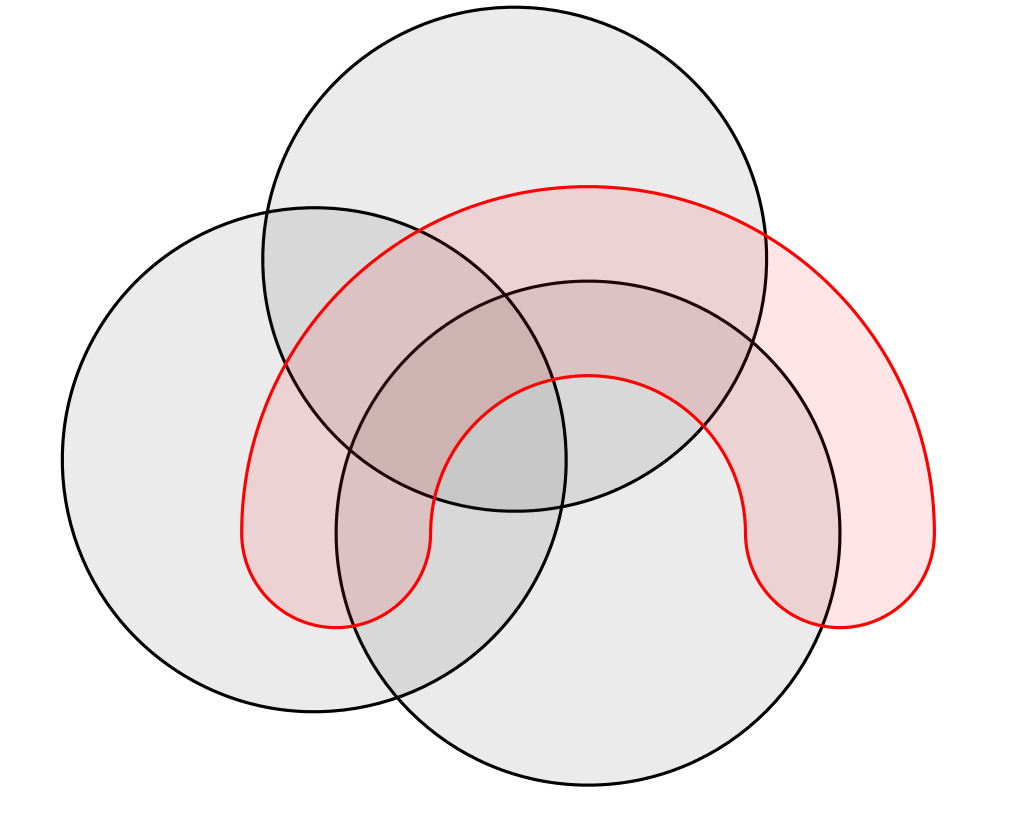
\includegraphics[width=6cm,height=5cm]{Venn4.png}
			\caption{Venn-Diagramm mit 4 Mengen}
		\end{figure}
	
	\section*{2.) $Beweisen$ $Sie:$}
		\subsection*{a) $\underbrace{\P(A)\cup\P(B)=\P(A\cup B)}_{**}:\Leftrightarrow A\subseteq B\vee B\subseteq A$}
		Für "$\Leftarrow$", zz. ist $\P(A)\cup\P(B)=\P(A\cup B)$.
			\begin{align*}
				&A\subseteq B\Rightarrow\underbrace{\P(A)\cup\P(B)=\P(B)}_{*}\text{ und }A\cup B=B\Rightarrow\P(A\cup B)=\P(B)\overset{*}{=}\P(A)\cup\P(B)\qed\\
				&\text{selbiges analog für }B\subseteq A.
			\end{align*}
		Für "$\Rightarrow$".
		\begin{align*}
			A\cup B\subseteq A\cup B&\Rightarrow B\cup A\in\P(A\cup B)&&&&&&&&&\\
			&\Leftrightarrow A\cup B\in\P(A)\cup\P(B)\\
			&\overset{**}{\Leftrightarrow} A\cup B\in\P(A)\vee A\cup B\in\P(B)\\
			&\Leftrightarrow A\cup B\subseteq A\vee A\cup B\subseteq B\\
			&\Leftrightarrow B\subset A\vee A\subset B\qed
		\end{align*}
	
		\subsection*{b) $\underbrace{\P(A)\Delta\P(B)\cap\P(A\Delta B)=\emptyset}_{(a)}:\Leftrightarrow \underbrace{A=B}_{(b)}$}
		(b)$\Rightarrow$(a):
			\begin{align*}
				&&&& (b)\Leftrightarrow \P(A)=\P(B) &\wedge A=B&&&&\\
				&\Rightarrow && &\P(A)\textbackslash\P(B)=\emptyset\wedge\P(B)\textbackslash\P(A)=\emptyset &\wedge A\textbackslash B=\emptyset\wedge B\textbackslash A=\emptyset&&&&\\
				&\Rightarrow && &\P(A)\textbackslash\P(B)\cup\P(B)\textbackslash\P(A)=\emptyset &\wedge\P(A\textbackslash B\cup B\textbackslash A)=\emptyset&&&&\\
				&\Rightarrow &&&\P(A)\Delta\P(B)=\emptyset &\wedge\P(A\Delta B)=\emptyset\qed&&&&
			\end{align*}
		(a)$\Rightarrow$(b)$\Leftrightarrow$$\neg$(b)$\Rightarrow\neg$(a):
			\begin{align*}
				&&&& (b)\Leftrightarrow \P(A)\neq\P(B) &\wedge A\neq B&&&&\\
				&\Rightarrow && &\P(A)\textbackslash\P(B)\neq\emptyset\wedge\P(B)\textbackslash\P(A)\neq\emptyset &\wedge A\textbackslash B\neq\emptyset\wedge B\textbackslash A\neq\emptyset&&&&\\
				&\Rightarrow && &\P(A)\textbackslash\P(B)\cup\P(B)\textbackslash\P(A)\neq\emptyset &\wedge\P(A\textbackslash B\cup B\textbackslash A)\neq\emptyset&&&&\\
				&\Rightarrow &&&\P(A)\Delta\P(B)\neq\emptyset &\wedge\P(A\Delta B)\neq\emptyset\qed&&&&
			\end{align*}
		\subsection*{c) $Wann$ $ist$ $\P(A)\cap\P(B)=\P(A\cap B)$ $?$}
			Seien $F,T$ Mengen.
			\begin{align*}
				&\text{Für $"\subseteq"$:} & &\text{Für $"\supseteq"$:}\\
				&\quad F\in\P(A)\cap\P(B) & &\quad T\in\P(A\cap B)\\
				&\quad F\in\P(A)\wedge F\in\P(B)& &\quad T\subseteq A\cap B\\
				&\quad F\subseteq A\wedge F\subseteq B& &\quad T\subseteq A\wedge T\subseteq B\\
				&\quad F\subseteq A\cap B& &\quad T\in \P(A)\wedge T\in\P(B)\\
				&\quad F\in\P(A\cap B)\qed& &\quad T\in\P(A)\cap\P(B)\qed\\
			\end{align*}
	\section*{3.) $Beweisen$ $Sie$ $durch$ $vollst\ddot andige$ $Induktion$ $f\ddot ur$ $alle$ $n\ge2$}

		\subsection*{a) $A_1\cap A_2\cap\dots\cap A_n=A_1\textbackslash[(A_1\textbackslash A_2)\cup(A_1\textbackslash A_3)\cup\dots\cup(A_1\textbackslash A_n)]$}
			\subsection*{$Induktionsanfang$} $falls:n=2$\\
			\scalebox{1.2}{\parbox{.5\linewidth}{%
					\begin{align*}
						A_1\cap A_2&=A_1\tb[(A_1\tb A_2)]\\
						x\in A_1\wedge x\in A_2&=x\in A_1\wedge x\notin A_1\tb A_2\\
						&=x\in A_1\wedge x\notin A_1\wedge\bar{A_2}\\
						&=x\in A_1\wedge x\in A_2\qed
					\end{align*}
			}}
			\subsection*{$Induktionsvoraussetzung$ $IV$}
			$mit:n=k,n\in\N$ $sei:$
			\scalebox{1.2}{\parbox{.5\linewidth}{%
					\begin{align*}
						A_1\cap A_2\cap\dots\cap A_k=A_1\textbackslash[(A_1\textbackslash A_2)\cup(A_1\textbackslash A_3)\cup\dots\cup(A_1\textbackslash A_k)]
					\end{align*}
			}}
			\subsection*{$Induktionsbehauptung$}
			$mit:n=k+1$ $sei:$
			\scalebox{1.2}{\parbox{.5\linewidth}{%
					\begin{align*}
						A_1\cap A_2\cap\dots\cap A_{k+1}=A_1\textbackslash[(A_1\textbackslash A_2)\cup(A_1\textbackslash A_3)\cup\dots\cup(A_1\textbackslash A_{k+1})]
					\end{align*}
			}}
			\subsection*{$Induktionsbeweis$}
			\scalebox{1.2}{\parbox{.5\linewidth}{%
					\begin{align*}
						A_1\cap A_2\cap\dots\cap A_{k+1}&\Leftrightarrow\emptyset\cup(A_1\cap A_2\cap A_3\cap\dots\cap A_{k+1})\\
						&\Leftrightarrow(A_1\cap \neg A_1)\cup(A_1\cap A_2\cap A_3\cap\dots\cap A_{k+1})\\
						&\overset{distr.}{\Longleftrightarrow}A_1\cap[\neg A_1\cup(A_2\cap A_3\cap\dots\cap A_{k+1})]\\
						&\overset{distr.}{\Longleftrightarrow}A_1\cap[(\neg A\cup A_2)\cap(\neg A_1\cup A_3)\cap\dots\cap (\neg A_1\cup A_{k+1})]\\
						&\overset{de Mor.}{\Longleftrightarrow}A_1\cap\neg[(A_1\cap \neg A_2)\cup(A_1\cap\neg A_3)\cup\dots\cup(A_1\cap\neg A_{k+1})]\\
						&\Leftrightarrow A_1\tb[(A_1\tb A_2)\cup(A_1\tb A_3)\cup\dots\cup(A_1\tb A_{k+1})]\qed
					\end{align*}
			}}
		\subsection*{b) $(A_1\textbackslash B_1)\cap(A_2\textbackslash B_2)\cap\dots\cap(A_n\textbackslash B_n)=(A_1\cap A_2\cap\dots\cap A_n)\textbackslash(B_1\cup B_2\cup\dots\cup B_n)$}
			\subsection*{$Induktionsanfang$ $f\ddot ur$ $n=2$ $gilt:$}
			\scalebox{1.2}{\parbox{.5\linewidth}{%
					\begin{align*}
						(A_1\tb B_1)\cap(A_2\tb B_2)&\Longleftrightarrow(A_1\cap\neg B_1)\cap(A_2\cap\neg B_2)\\
						&\overset{kommu.}{\Longleftrightarrow}(A_1\cap A_2)\cap(\neg B_1\cap\neg B_2)\\
						&\overset{deMor.}{\Longleftrightarrow}(A_1\cap A_2)\cap\neg(B_1\cup B_2)\\
						&\Leftrightarrow(A_1\cap A_2)\tb(B_1\cup B_2)\qed
					\end{align*}
			}}
			\subsection*{$Induktionsvoraussetzung$ $IV$}
			$mit:n=k,n\in\N$ $gilt:$\\
			\scalebox{1.2}{\parbox{.5\linewidth}{%
					\begin{align*}
						(A_1\tb B_1)\cap(A_2\tb B_2)\cap\dots\cap(A_k\tb B_k)=(A_1\cap A_2\cap\dots\cap A_k)\tb(B_1\cup B_2\cup\dots\cup B_k)
					\end{align*}
			}}
			\subsection*{$Induktionsbehauptung$}
			$mit:n=k+1$ $soll gelten:$\\
			\scalebox{1.2}{\parbox{.5\linewidth}{%
					\begin{align*}
						(A_1\tb B_1)\cap(A_2\tb B_2)\cap\dots\cap(A_{k+1}\tb B_{k+1})=(A_1\cap A_2\cap\dots\cap A_{k+1})\tb(B_1\cup B_2\cup\dots\cup B_{k+1})
					\end{align*}
			}}
			\subsection*{$Induktionsbeweis$}
			\scalebox{1.2}{\parbox{.5\linewidth}{%
					\begin{align*}
						(A_1\tb B_1)\cap(A_2\tb B_{k+1})\cap\dots\cap(A_{k+1}\tb B_n)&\Leftrightarrow(A_1\cap\neg B_1)\cap(A_2\cap\neg B_2)\cap\dots\cap(A_{k+1}\cap\neg B_{k+1})\\
						&\overset{komm.}{\Longleftrightarrow}(A_1\cap A_2\cap\dots\cap A_{k+1})\cap(\neg B_1\cap\neg B_2\cap\dots\cap\neg B_{k+1})\\
						&\Longleftrightarrow (A_1\cap A_2\cap\dots\cap A_{k+1})\tb(B_1\cup B_2\cup\dots\cup B_{k+1})\qed
					\end{align*}
			}}
\end{document}
